\documentclass[conference]{IEEEtran}
\IEEEoverridecommandlockouts
% The preceding line is only needed to identify funding in the first footnote. If that is unneeded, please comment it out.
\usepackage{cite}
\usepackage{amsmath,amssymb,amsfonts}
\usepackage{algorithmic}
\usepackage{graphicx}
\usepackage{textcomp}
\usepackage{xcolor}
\usepackage{listings}
\graphicspath{ {./naibaoimage/} }
\def\BibTeX{{\rm B\kern-.05em{\sc i\kern-.025em b}\kern-.08em
    T\kern-.1667em\lower.7ex\hbox{E}\kern-.125emX}}
\begin{document}

\title{Paper Title*\\
{\footnotesize \textsuperscript{*}Note: Sub-titles are not captured in Xplore and
should not be used}
\thanks{Identify applicable funding agency here. If none, delete this.}
}

\author{\IEEEauthorblockN{1\textsuperscript{st} Given Name Surname}
\IEEEauthorblockA{\textit{dept. name of organization (of Aff.)} \\
\textit{name of organization (of Aff.)}\\
City, Country \\
email address}
\and
\IEEEauthorblockN{2\textsuperscript{nd} Given Name Surname}
\IEEEauthorblockA{\textit{dept. name of organization (of Aff.)} \\
\textit{name of organization (of Aff.)}\\
City, Country \\
email address}
\and
\IEEEauthorblockN{3\textsuperscript{rd} Given Name Surname}
\IEEEauthorblockA{\textit{dept. name of organization (of Aff.)} \\
\textit{name of organization (of Aff.)}\\
City, Country \\
email address}
\and
\IEEEauthorblockN{4\textsuperscript{th} Given Name Surname}
\IEEEauthorblockA{\textit{dept. name of organization (of Aff.)} \\
\textit{name of organization (of Aff.)}\\
City, Country \\
email address}
\and
\IEEEauthorblockN{5\textsuperscript{th} Given Name Surname}
\IEEEauthorblockA{\textit{dept. name of organization (of Aff.)} \\
\textit{name of organization (of Aff.)}\\
City, Country \\
email address}
\and
\IEEEauthorblockN{6\textsuperscript{th} Given Name Surname}
\IEEEauthorblockA{\textit{dept. name of organization (of Aff.)} \\
\textit{name of organization (of Aff.)}\\
City, Country \\
email address}
}

\maketitle

\begin{abstract}
This document is a model and instructions for \LaTeX.
This and the IEEEtran.cls file define the components of your paper [title, text, heads, etc.]. *CRITICAL: Do Not Use Symbols, Special Characters, Footnotes, 
or Math in Paper Title or Abstract.
\end{abstract}

\begin{IEEEkeywords}
component, formatting, style, styling, insert
\end{IEEEkeywords}
For papers published in translation journals, please give the English 
citation first, followed by the original foreign-language citation \cite{b6}.

\section{Background}
\subsection{Triangle mesh}
Triange mesh is a kind of polygon mesh. Polygon mesh is also called "Mesh",it's a data structure used in computer graphics to model various irregular objects. In the real world,the surface of objects is intuitively composed of curved surfaces, but in the computer world, however, only discrete structures can be used to simulate continuous things in reality. So the curved surface in the real world is actually composed of countless small polygon patches in the computer. For example, the model in the Fig.\ref{Triangle Mesh_sphere_surface}. 
\begin{figure}[ht]
    \caption{Example of Triangle Mesh}
    \label{Triangle Mesh_sphere_surface}
    \centering 
    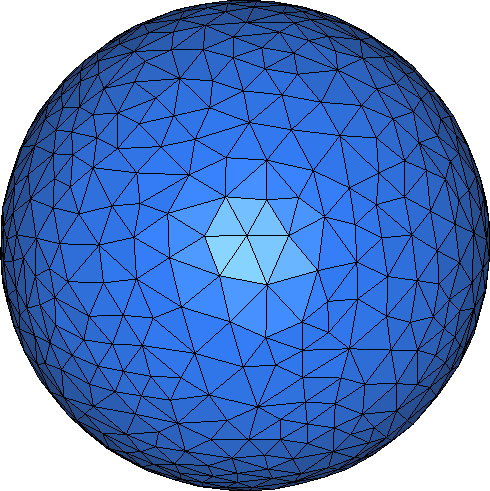
\includegraphics[width=4cm]{Triangle Mesh_sphere_surface.png}
\end{figure}

In fact, a large number of small triangles are used inside the computer to form such a shape. Such a collection of facets is called Mesh. Mesh can be composed of triangles or other plane shapes such as quadrilaterals, pentagons, etc.; Because of all the plane polygons can also be subdivided into triangles, it's also general to use a triangle mesh composed of triangles to represent the surface of an object.

For the Triangle Mesh, most of kenrels use indices and vertex to set the data of Triangle, not all the Triangle needs 3 vertexs, because it can be connected with pther triangle, so we need to set the vertex data. And a triangle whose vertices are laid out counter-clockwise has its geometry normal pointing upwards outside the front face, we use indice to contral counter-clockwise or clockwise.

\subsection{BVH}
A bounding volume hierarchy (BVH) is a tree structure on a set of geometric objects. 
All geometric objects are wrapped in bounding volumes that form the leaf nodes of the tree. 
These nodes are then grouped as small sets and enclosed within larger bounding volumes. 
These, in turn, are also grouped and enclosed within other larger bounding volumes in a recursive fashion, 
eventually resulting in a tree structure with a single bounding volume at the top of the tree. 
Bounding volume hierarchies are used to support several operations on sets of geometric objects efficiently, 
such as in collision detection and ray tracing \cite{Bounding_volume_hierarchy}.

\begin{figure}[h]
\caption{Example of BVH Tree}
\label{Example of BVH Tree}
\centering 
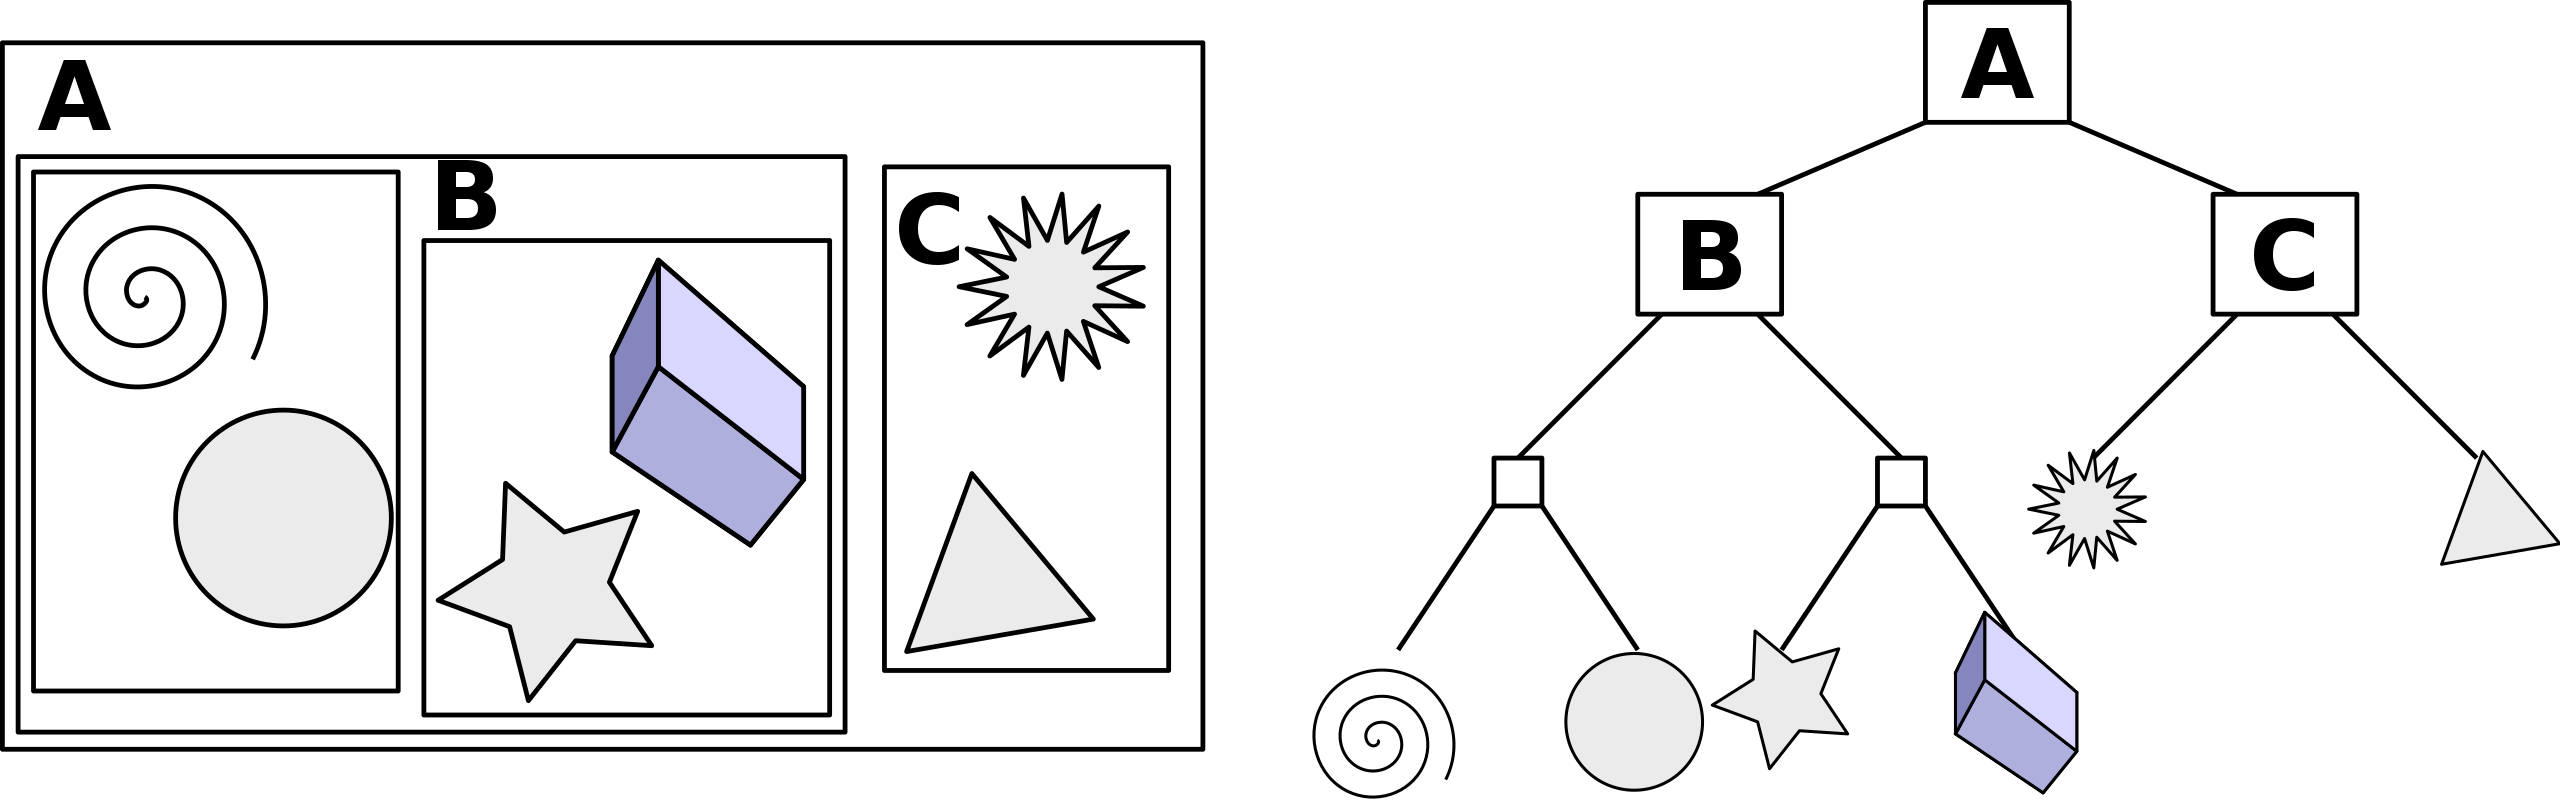
\includegraphics[width=8cm]{Example_of_bounding_volume_hierarchy_svg.png}
\end{figure}

For example, when we implement Snell's law in Python, when calculating multiple geometry or planes, we tested for 2D scene, for complexing 3D scene, we need to
use a algorithm called AABB. 
the method we used is to let the ray operate with each graph to calculate the intersection point, 
and then determine its true intersection point, so algorithmic complexity is n. And we use a tree structure to manage graphics, 
which can reduce the complexity to $log (n)$.

Using BVH requires two stages of work to be considered: Build and Traversal.
The construction work considers how to construct a binary tree that can effectively describe the current scene information. 
The key to this is how to divide assumed all objects scattered randomly in the scene Partition, that is, 
decide which objects should be divided into the left subtree and which objects should be divided into the right subtree. 
 
The best way is called Surface Area Heuristic, also SAH, the SAH algorithm calculates the mean value of the 
average complexity based on the size of the surface area and the direction of the rays, 
thereby dividing the BVH tree into the structure with the lowest mean value.

First select an axis with the largest divergence in the graphic distribution, and then spilt it equally along the axis in space, 
Fig.\ref{Example of SAH Spilt}. shows two different scheme spilting, and traversal all of scheme to find the best one.
\begin{figure}[ht]
    \caption{Example of SAH Spilt}
    \centering 
    \label{Example of SAH Spilt}
    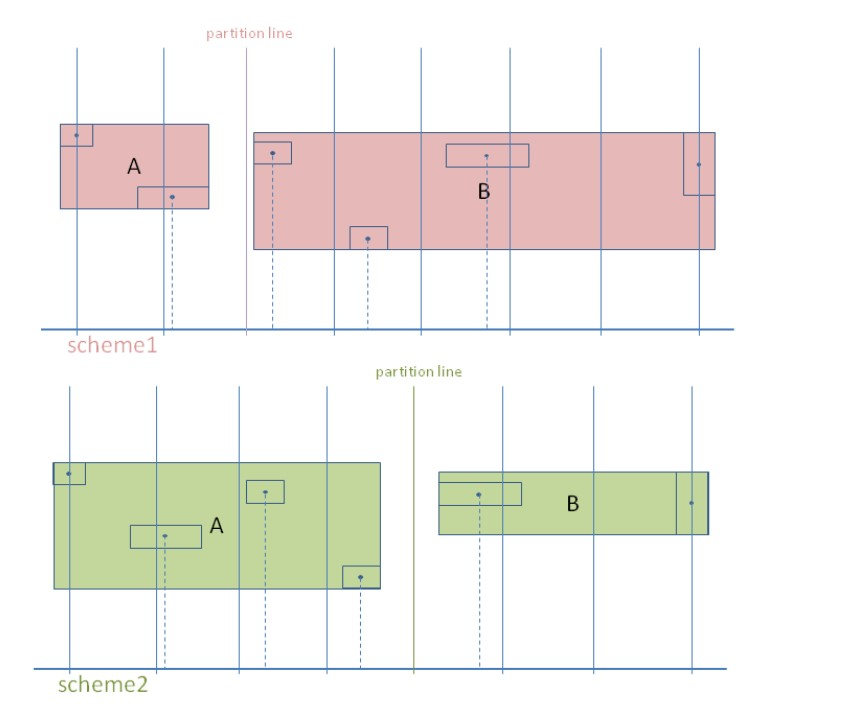
\includegraphics[width=8cm]{Example_SAH_Spilt.jpg}
\end{figure}


SAH does not completely "non-overlap" or make the distribution after partitioning "uniform", like Fig.\ref{Example of Spilt}.
\begin{figure}[ht]
    \caption{Example of Spilt}
    \label{Example of Spilt}
    \centering 
    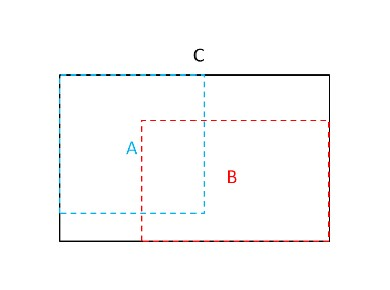
\includegraphics[width=8cm]{Example_Spilt.jpg}
\end{figure}
but each time it makes a partition, it chooses the best plan under the current situation. So it is called a Heuristic algorithm.


\subsection{About the tools}
\paragraph{Python}

Python is an interpreted, high-level, general-purpose programming language. 
Created by Guido van Rossum and first released in 1991, Python's design philosophy emphasizes code readability with its notable use of significant whitespace. 
Its language constructs and object-oriented approach aim to help programmers write clear, logical code for small and large-scale projects.\cite{python1}

Compared to C++, Python has a simpler syntax,and Python also has many extension packages. such as Numpy,it can be used to calculate vectors directly,
Sympy can also be used to solve equations with symbol. By importing those packages, we don't need to overload the operator for vectors calculating, and we don't need to
solve some complex equations by ourselves.

In addition, Python also supports interactive shells, such as ipython, which is very friendly to beginners in programming, 
can speed up our language learning speed, and greatly improve our debugging capabilities.

\paragraph{C++}
Although Python is very convenient for mathematical operations and friendly enough for beginners, but
Python has cross-platform packaging problems and the performance is not good enough. 
Therefore, projects with huge calculations such as ray tracing generally use better performance 
and Better use of programming languages with different data structures, such as C++.

\paragraph{Embree}
Intel® Embree is a collection of high-performance ray tracing kernels, developed at Intel. 
The target users of Intel® Embree are graphics application engineers who want to improve the 
performance of their photo-realistic rendering application by leveraging Embree's performance-optimized ray tracing kernels. 
The single-ray traversal kernels of Intel® Embree provide high performance for incoherent workloads and are very easy to integrate into existing rendering applications.
Using the stream kernels, even higher performance for incoherent rays is possible, but integration might require significant code changes to the application to use the stream paradigm. 
In general for coherent workloads, the stream mode with coherent flag set gives the best performance.
Intel® Embree also supports dynamic scenes by implementing high-performance two-level spatial index structure construction algorithms. \cite{Intel_Embree}

Embree is compiling with C++, and we can use Embree API to realise Raytracing.

\section{Simulation Design}

\subsection{The use of Embree}
\paragraph{Compiling Embree}
We compiled Embree on Ubuntu, and installed the release version of Embree on the Windows platform. Our embree-based program was developed on Windows platform. The official recommendation is that using Cmake to compile to generate project files on different platforms. For our Windows Platform, we use Visual Studio as IDE to compile our project.
\paragraph{Embree API}
For the simplest case, we should at lest have a Device object, Scene object and Geometry object. 
\begin{itemize}
    \item Device object: it allows different components of the application to use the Embree API without interfering with each other. 
    \item Scene object: it's a container for a set of geometries, and contains a spatial acceleration structure which can be used to perform different types of rayqueries.
    \item Geometry object: it depends on geometry type, like triangle mesh. 
\end{itemize}
\paragraph{Our Demo}
We refer to the official tutorial and the official API to achieve a hit of ray and scene. The scene contains 8 triangule mesh, and we have 2 rays.
\begin{figure}[ht]
    \caption{Triangle location}
    \label{Triangle_Location}
    \centering 
    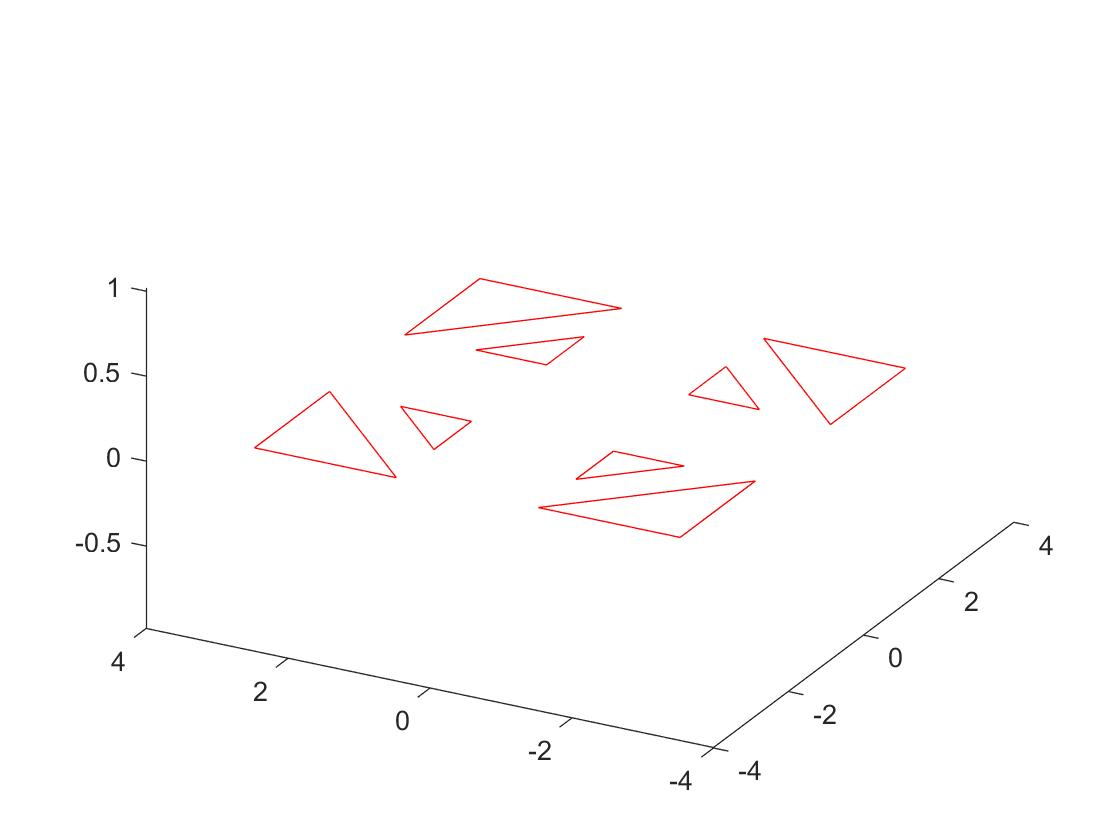
\includegraphics[width=8cm]{Triangle_Location.jpg}
\end{figure}

We are not using BVH Tree , so the complexity of Intersect's algorithm is $o(n)$. At the same time, we calculated the running time of the program, although there are millisecond tolerance, the accuracy is sufficient.

\section{Result}
\subsection{Embree Demo}
\paragraph{Our Demo}
We just print the result in Command, there is no image output.

Single ray structure are define in this structure, it's also in Embree API.
\lstset{language=C++}
\begin{lstlisting}
    #include <embree3/rtcore_ray.h>
    struct RTC_ALIGN(16) RTCRay
    { 
        float org_x; 
        float org_y; 
        float org_z; 
        float tnear; 
        float dir_x; 
        float dir_y; 
        float dir_z; 
        float time; 
        float tfar;  
        unsigned int mask; 
        unsigned int id;  
        unsigned int flags; 
    };
\end{lstlisting}
the ray's org is the coordinate of ray origin. and geometry 0 is the gemoetry ID of our gemoetry object, primitive is ID of our triangle, base on our indices buffer, tfar is end of ray segment. 

From Fig.\ref{Demo_Result} we can see two rays hit 2 Trianges, and the program run time is 17ms.
\begin{figure}[ht]
    \caption{Demo Result}
    \label{Demo_Result}
    \centering 
    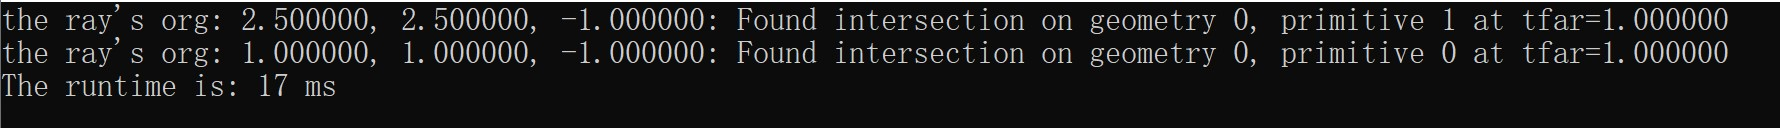
\includegraphics[width=8cm]{Demo_Result.jpg}
\end{figure}
\paragraph{BVH Result}
Embree's Tutorial give us a Demo to show the performance of BVH with SAH.

The result is:
\begin{figure}[ht]
    \caption{BVH Result}
    \label{BVH_Result}
    \centering 
    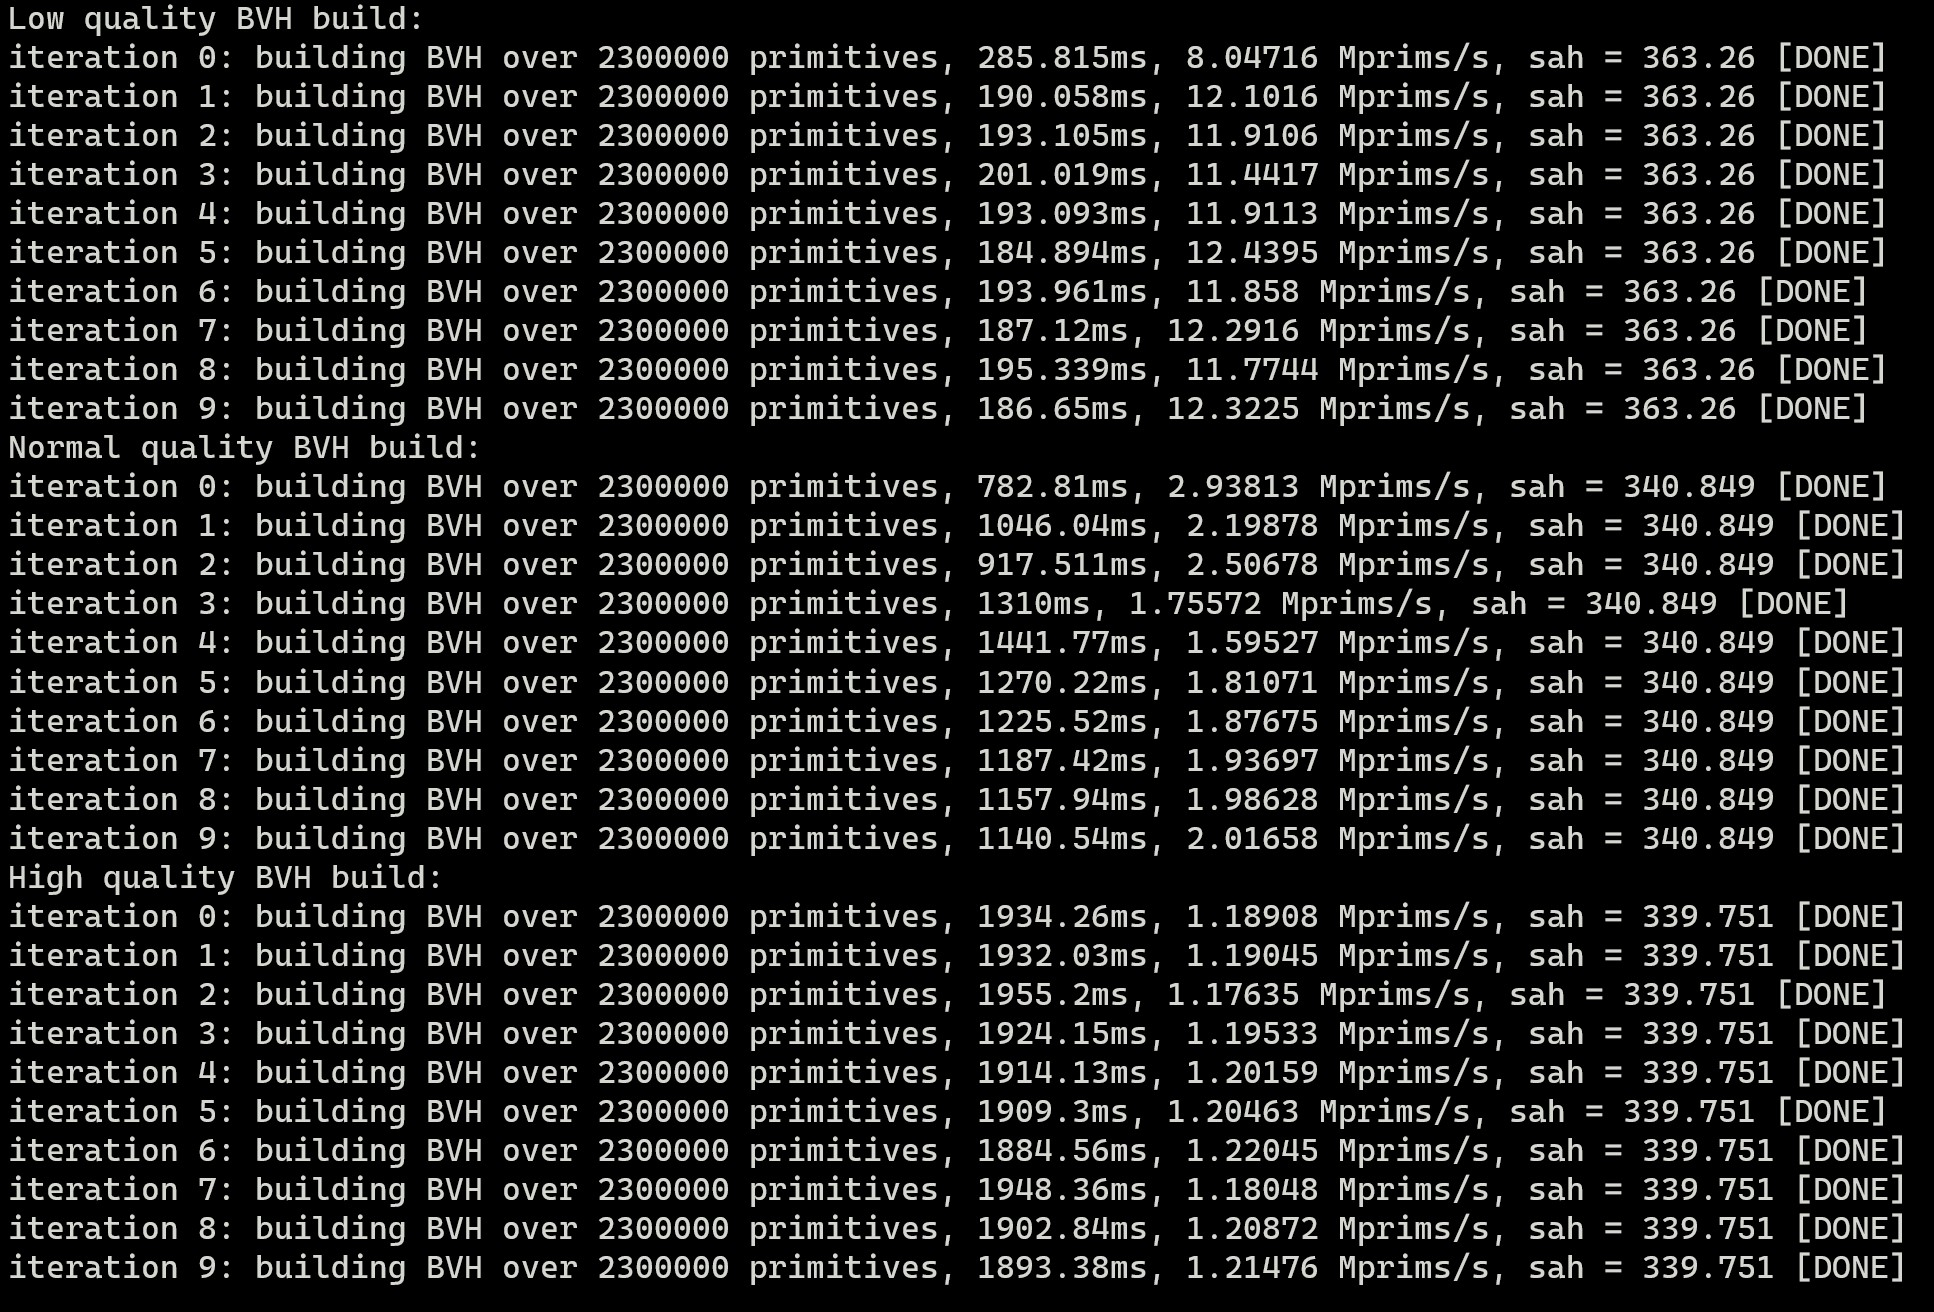
\includegraphics[width=8cm]{BVH_Result.jpg}
\end{figure}

from Fig.\ref{BVH_Result} we can see, it has over 2300000 primiteves, and the run time is base on the quality is between 200ms and 2000ms, in our demo, we 
only have 8 simple triangle primitives, and the run time is 17ms. so we can find that BVH is very fast.

\bibliographystyle{./bibliography/IEEEtran}
\bibliography{./bibliography/IEEEabrv,./bibliography/IEEEexample,./bibliography/Naibao}



\end{document}
